\documentclass{standalone}
\usepackage{amsmath}
\usepackage{tikz}
\begin{document}
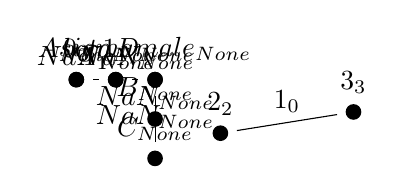
\begin{tikzpicture}
\node[fill=black, circle, inner sep=2pt, label=above:{\textcolor{black}{$0_{0}$}}] (G1N0) at (3.7,-0.2) {};
\node[fill=black, circle, inner sep=2pt, label=above:{\textcolor{black}{$1_{1}$}}] (G1N1) at (4.2,-0.2) {};
\node[fill=black, circle, inner sep=2pt, label=above:{\textcolor{black}{$sigma male_{None}$}}] (G1Nsigma male) at (4.7,-0.2) {};
\node[fill=black, circle, inner sep=2pt, label=above:{\textcolor{black}{$2_{2}$}}] (G1N2) at (5.53,-0.88) {};
\node[fill=black, circle, inner sep=2pt, label=above:{\textcolor{black}{$3_{3}$}}] (G1N3) at (7.22,-0.61) {};
\draw[draw=black, shorten >=3pt, shorten <=3pt] (G1N0) -- (G1N1) node[midway, above] {\textcolor{black}{$1_{1}$}};
\draw[draw=black, shorten >=3pt, shorten <=3pt] (G1N1) -- (G1Nsigma male) node[midway, above] {\textcolor{black}{$NaN_{None}$}};
\draw[draw=black, shorten >=3pt, shorten <=3pt] (G1N2) -- (G1N3) node[midway, above] {\textcolor{black}{$1_{0}$}};
\node[fill=black, circle, inner sep=2pt, label=above:{\textcolor{black}{$A_{None}$}}] (G2NA) at (3.7,-0.2) {};
\node[fill=black, circle, inner sep=2pt, label=above:{\textcolor{black}{$beta_{None}$}}] (G2Nbeta) at (4.2,-0.2) {};
\node[fill=black, circle, inner sep=2pt, label=above:{\textcolor{black}{$D_{None}$}}] (G2ND) at (4.7,-0.2) {};
\node[fill=black, circle, inner sep=2pt, label=above:{\textcolor{black}{$B_{None}$}}] (G2NB) at (4.7,-0.7) {};
\node[fill=black, circle, inner sep=2pt, label=above:{\textcolor{black}{$C_{None}$}}] (G2NC) at (4.7,-1.2) {};
\draw[draw=black, shorten >=3pt, shorten <=3pt] (G2NA) -- (G2Nbeta) node[midway, above] {\textcolor{black}{$NaN_{None}$}};
\draw[draw=black, shorten >=3pt, shorten <=3pt] (G2NB) -- (G2NC) node[midway, above] {\textcolor{black}{$NaN_{None}$}};
\draw[draw=black, shorten >=3pt, shorten <=3pt] (G2NC) -- (G2ND) node[midway, above] {\textcolor{black}{$NaN_{None}$}};
\end{tikzpicture}
\end{document}
